
\begin{refsection}

\chapter{Introduction}

The importance of non-bonding interactions in our world simply cannot be overstated.
While we may think of the more familiar covalent and ionic bonds as the core of chemistry, more often than not it is non-bonding interactions that dictate the nature of substances, from bulk properties such as tensile strength, to microscopic phenomena like protein-ligand interactions.

At a fundamental level, all non-bonding interactions (indeed, conventional bonding too) are attributable to the electrostatic force.
However, it is more convenient to broadly categorise interactions based on strength and structural motifs that are common to each class.
Such classes include dispersion forces, dipole-dipole interactions, and H-bonding.
In the 19th century, it became apparent that these classes paint an incomplete picture of intermolecular bonding.
As part of their investigation into solvent effects on the colour of iodine solutions in 1949, Bensei and Hildebrand invoked the concept of ``charge-transfer'' complexes to explain the association of molecular iodine with nucleophililc solvent molecules.\autocite{Benesi1949}
Although the electrophilic nature of molecular halogens was already well appreciated with respect to reactivity, this appears to be the first acknowledgement that this understanding could be applied to ground state complexes.
In support of this, Hassel and Hvoslef elucidated the structure of a 1:1 complex of molecular bromine and 1,4-dioxane in 1954, and observed an unusally strong interaction between the two molecules.\autocite{Hassel1954}
The crystal was comprised of long chains of monomers (\cref{fig:hassel-xray}), exhibiting a very short O\dots Br contact (2.71\AA, the sum of the VDW radii is 3.37\AA), and a slightly lengthened Br--Br bond (2.31\AA~vs 2.28\AA~in gaseous bromine).

\begin{figure}[ht]
  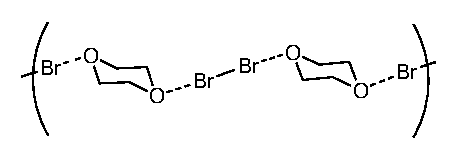
\includegraphics[width=0.6\columnwidth]{Figures/hassel-xray.eps}
  \caption{Long chains of molecular bromine and 1,4-dioxane, observed by Hassel and Hvoslef.}
  \label{fig:hassel-xray}
\end{figure}

In the subsequent years, a wide variety of names and labels were applied to the ``charge-transfer'' phenomenon, including ``lock and key'', ``donor-acceptor'', and ``filling of antibonding orbitals'', as summarised in Bent's excellent 1968 review\autocite{Bent1968}.
The term ``halogen bonding'' (X-bonding) only gained widespread acceptance in 1983 after the publication of the review of Dumas, Gomel, and Guerin.\autocite{Dumas1983}
The term deliberately evokes similarity to the better known concept of hydrogen bonding, as the two phenomena are of comparable strength and, importantly, directionality.
In 1998 Anthony C. Legon again used the term to describe the attractive interaction between halogens and Lewis bases in prereactive complexes, harking back to the original understanding of electrophilic halogens as a primarily reactive phenomenon.\autocite{Legon1998,Legon1999}
In the following years, the potential of X-bonding was more fully recognised, with applications in supramolecular chemistry and self-assembly\autocite{Corradi2000,Metrangolo2008,Priimagi2013}, catalysis and bond activation\autocite{Walter2011,Soloshonok2017,Takagi2017}, and molecular sensing and recognition\autocite{Cornes2017,VargasJentzsch2013,Borissov2017}.

From X-bonding grew the related concepts of chalcogen (Ch-), pnicogen (Pn-), and tetrel bonding (T-bonding), as the electrophilic nature of these elements was discovered.\autocite{Murray2007}
Similar applications have also been found for these classes of noncovalent interactions, Ch-bonding in particular.\autocite{Fanfrlik2014,Garrett2016,Ho2016,Wonner2017,Mitchell2017,Benz2017,Biot2018,Ho2017}

\section{Chalcogen Bonding}
Ch-bonding is the attractive interaction between a Lewis base and a chalcogen atom bearing an electron withdrawing substituent.
The terminology of Ch-bonding partners is perhaps counterintuitive, as donors and acceptors are named by analogy with H-bonded equivalents.
Note this is contrary to the formal flow of electron density; Ch-bond \emph{donors} bear vacant \emph{acceptor} orbitals, while Ch-bond \emph{acceptors} are \emph{donors} of electron density.
For the purposes of this report, ``donor'' will refer to the Lewis acidic chalcogen species.

\subsection{Mechanisms}
As was discussed in the introduction, all intermolecular (and indeed \emph{intra}molecular) forces are manifestations of the electromagnetic force.
Nonetheless, it is more convenient to categorise energetic contributions to any given interaction as orbital, electrostatic, or dispersion mediated, as there are marked differences in strength and directionality between them.
Historically, X- and Ch-bond interactions were understood to be primarily due to orbital overlap and resulting charge transfer.
Evidence for this included the lengthening of the X--X bond corresponding to increased occupation of the $\sigma^{\star}$(X-X) orbital due to the incoming lone pair (this was observed in Hassel and Hvoslef's original work\autocite{Hassel1954}).
Characteristic charge transfer bands are also observed in the UV-vis spectra of halogen solutions.\autocite{Blackstock1987}

Such evidence of orbital contributions is not, however, common to all systems displaying X- or Ch-bond interactions.
The iodoperfluoroalkanes and arenes studied by Resnati et al show no charge transfer bands in UV-vis spectra, yet are exceptionally strong X-bond donors.\autocite{Yan2014}
Jane Murray and Peter Politzer have advocated for an alternative, primarily electrostatic explanation of X- and Ch-bond interactions.\autocite{Murray2008,Murray2009}
They propose that a positively charged $\sigma$-hole is generated along the extension of a $\sigma$ bond to an electron withdrawing substituent, due to polarisation of the bonding orbital.
This also adequately explains the strength and directionality of these interactions.

An interpretation which has not attracted as much attention is that of dispersion forces.

While the varying contributions from each of these factors can be dissected computationally via pertubation methods, experimental evidence is surprisingly sparse.
Pascoe, Ling and Cockroft, however, devised an elegant experiment to quantitatively determine energetic contributions.\autocite{Pascoe2017}
\textsuperscript{19}F NMR was used to determine the relative populations of two conformors of a "molecular balance", one bearing a Ch-bond interaction, one not.
Interaction energies were thus derived, and found to be more or less invariant with respect to the solvent.
This appeared to rule out electrostatic contributions, as solvent dipole moment and bulk polarisability would otherwise have a large effect on the position of the equilibrium.
These results also suggest that dispersion plays only a minor role, for similar reasons.

DFT was used to further probe the dispersion contribution.
Free energies were calculated using functionals which both did, and did not include dispersion corrections, and the values compared to the experimental results.
The non-dispersion corrected B3LYP functional gave superior correlation with experiment than did either M06-2X and $\omega$B97-D, both of which include dispersion.
This provided additional evidence that, in the systems studied, the major contributor to the interaction is orbital overlap and charge transfer.

Although current evidence points towards these interactions being primarily orbital related, the electrostatic ``$\sigma$-hole'' terminology of Politzer and Murray has stuck, and the term is now used to encompass the whole gamut of X- Ch- Pn- and T-bonding interactions.

\section{Applications of Ch-Bonding}
Ch-bonding, and by extension, all $\sigma$-hole interactions can theoretically be applied to any formal Lewis acid-base system.
They are especially attractive as a hydro\emph{phobic} complement to H-bonding interactions, which are generally considered to be hydro\emph{philic}.
The following are brief summaries of existing applications in the literature.

\subsection{Materials}
The major applications of $\sigma$-hole interactions have so far been in the realm of crystal engineering.
Early work by Corradi et al showed that halogen bonding was able to outcompete H-bonding in the formation of supramolecular architectures.\autocite{Corradi2000}
A review by Metrangolo summarised the forms that are accessible using X-bonding to direct crystal growth.\autocite{Metrangolo2008}
1D, 2D, and 3D architectures are able to be generated using appropriate X-bond donors, and these show potential in the design of liquid crystals, organic semiconductors and paramagnetic materials.
A more recent review by the same group described applications in anion transport, and luminescent and photoresponsive crystals.\autocite{Priimagi2013}
The group of Stefan Matile has further explored anion transport, and has published a review comparing X-bonding with other hydrophobic interactions such as anion-$\pi$ and anion-macrodipole interactions.\autocite{VargasJentzsch2013}

Ch-bonding, too, has been investigated with respect to materials chemistry.
Fanfrlik et al demonstrated the importance of Ch-bonding on the crystal packing of thiaboranes.\autocite{Fanfrlik2014}
They found that the sulfur-based $\sigma$-hole was sufficiently strong to interact with the weakly basic $\pi$ electrons of a phenyl group, with contacts as short as 3.2\AA~being observed.

In 2016, Ho et al published their work into tellurium-based Ch-bonding.\autocite{Ho2016}
Their scaffolds are based on an iso-tellurazole N-oxide, which reversibly forms macrocyclic structures that persist in both gas and solution phase.
The macrocycles were found to coordinate \ce{Pd2+}.
This is particularly interesting, as the tellurium atoms are simultaneously behaving as a Lewis acid and base.
The authors point out that such soft macrocycles are quite rare, and their work could facilitate further studies of transition metals in a soft coordination environment.
They went on to investigate benzo-fused derivatives of iso-tellurazoles, as well as selenium analogues, which crystallised to form macromolecular pores and voids.\autocite{Ho2017}

The Taylor group has been active in the development of X- and Ch-bonding molecular sensors.
Early work demonstrated that X-bonding tridentate ligands (reminiscent of enterobactin) showed moderate selectivity for \ce{Cl-}.\autocite{Dimitrijevic2010}
They later developed bidentate Ch-bonding ligands which exhibited a tenfold increase in association constant with respect to chloride.\autocite{Garrett2015a,Garrett2016}

Similar results have been achieved by the Beer group, who have developed X-bonding sensors for the perrhenate anion.\autocite{Cornes2017}
These sensors are based on functionalised cyclodextrins, and are even more sensitive than the corresponding H-bonding analogues.
The group has also use iodotriazole scaffolds to chelate anions.\autocite{Borissov2017}
Incorporation of a chial binapthol moiety was shown to differentiate between enantiomers of chiral anions.

The role of selenium-based Ch-bonding on the crystal structure and mechanism of the drug ebselen was demonstrated by Thomas et al.\autocite{Thomas2015}
Interestingly, the Lewis acidity of the $\sigma$-hole was invoked as an explanation of the antioxidant properties of the drug.

\subsection{Catalysis and bond activation}
In 2008, halogen bonding was first applied to a Hantzsch ester reduction of a quinoline derivative.\autocite{Bruckmann2008}
This reaction is well characterised and understood, and has been catalyzed with a variety of Br\o nsted and Lewis acids.
The X-bond donors chosen were perfluoroiodoalkanes, and high conversions were achieved with modest catalyst loadings of 10\%.

In 2011, a modified Ritter reaction was devised wherein benzhydryl bromide was activated by a dicationic imidazolium-based X-bond donor to give the carbocation intermediate, which was then captured by acetonitrile and then hydrolysed to afford the amide product.\autocite{Walter2011}
This pioneering work was limited by the necessity of stoichiometric amounts of the X-bond donor, as it is consumed in the course of the reaction.

A similar alkylation of 1-chloroisochroman was achieved by the same group using a neutral perfluoroiodoarene X-bond donor in catalytic quantities.\autocite{Kniep2013}
The proposed mechanism is similar to the thiourea-catalysed reaction of Reisman, Doyle, and Jacobsen\autocite{Reisman2008}, which has shown promise in asymmetric induction.
The authors noted issues with solubility of the perfluoroiodoarene catalysts, which is expected of such highly fluorinated compounds.

These reactions have all been repeated with Ch-bond donors in place of X-bonds.

The quinoline reduction was sucessfully catalysed by a dithiophene system by Benz et al. in 2017\autocite{Benz2017}, and then again by the same group with a benzodiselenazole.\autocite{Benz2017a}
With the increased selectivity and strength of the Se-based Ch-bonding catalyst compared to the X-bonding perfluoroiodoalkane, the authors were able to reduce the catalyst loading to 1\%.

Wonner et al developed a selenated bisbenzimidazolium Ch-bonding catalyst for the alkylation of 1-chloroisochroman, and solvolysis of benzyhydryl bromide.\autocite{Wonner2017,Wonner2017a}
Although the best results were observed with the dicationic catalysts, conversion was also achieved with a neutral bisbenzimidazole catalyst, providing further evidence that the catalytic Lewis-acid site is indeed the $\sigma$-hole.
For a given row in the periodic table (i.e. comparing a Se-based donor to a Br-based donor), Ch-bonding appeared to give superior results to X-bonding, as measured by \% yield.

An unusal manifestation of X-bonding is in the self-disproportionation of enantiomers, as reported by Terada et al.\autocite{Soloshonok2017}
They observed spontaneous enrichment of one enantiomer of mebroqualone upon chromatography using an achiral solid phase, which they attributed to the formation of diasteromeric X-bonded oligomers.
This phenomenon has been observed in compounds capable of interacting through H-bonding or strong dipole-dipole interactions.

\subsection{Biological systems}

\subsubsection{Proteins}
While we usually think of the tertiary structure of proteins as being dominated by H-bonding and hydrophobic effects, there is increasing evidence that Ch-bonding plays an important role as well.
This is not unexpected, as sulfur, a component of both cysteine and methionine, is known to form Ch-bonds in small molecules.
In the early days of Ch-bonding interactions (2001, before the name had come into common use) Iwaoka et al published an analysis of 604 protein structures in the Protein Data Bank (PDB).\autocite{Iwaoka2001}

A remarkable number of close contacts (sum of Van der Waals radii plus 0.5\AA) between sulfur and Lewis basic (X) atoms were identified in the structures, with 33\% of cysteine residues and 22\% of methionine residues showing a close contact.
Furthermore, the geometric parameters of these contacts were studied, with more than half of all contacts having a S--S--X (X=O,N) of 150--180\degree.
The observed contacts were ascribed to a $\pi$(C=O)$\rightarrow \sigma^{\star}$(S--S) interaction, in contrast to the $n(X) \rightarrow \sigma^{\star}$(S-X) interaction which dominates in small molecules.
Also contrary to the case of small molecules, the authors suggest that the orbital component of the interaction is small, though important for establishing the directionality of the interaction.
Dispersion appears to be the major stabilising force, as optimization using a non-dispersion corrected level of theory gave unrealistically large distances.

The differences between Ch-bonding in proteins and small molecules is likely due to variation in orbital energies in the functional groups which are found in each class.
While small molecule Ch-bond donors are characterised by easily accessible, low energy $\sigma^{\star}$(Ch--X) orbitals, these are simply not found in proteins.
Instead, donors are characterised by $\sigma^{\star}$(S--S) or $\sigma^{\star}$(S--C) orbitals, which are much higher in energy and less accessible to acceptors.
Ch-bond acceptors, too, are markedly different between small molecules and proteins.
In general, the HOMO of a system (the most Lewis basic site) is dominated by lone pairs.
This is observed in most small molecules, as they form Ch-bonds through these lone pairs.
However, the amide bond, which is ubiquitous in proteins, shows an unusual inversion in orbital energies.
The $\pi$(C=O) orbital is elevated with respect to the lone pair according to MP2 calculations, making it the more basic site.
Structural data supports this assertion, as the Ch-bond donor usually approaches the top of the C=O bond in proteins, rather than the usual approach towards the oxygen lone pair.\autocite{Iwaoka2012}

It is worth noting that selenium is also found in proteins as selenocysteine and selenomethionine.
This would be expected to be an even stronger Ch-bond donor.
However, selenoproteins are relatively few in number, precluding such extensive statistical analysis.\autocite{Iwaoka2015}
They are only mentioned here for the sake of completeness.

\emph{Intra}molecular interactions are just one instance of Ch-bonding in biological systems.
Proteins often interact with ligands or substrates through H-bonds, so it is reasonable to propose that Ch-bonding could be applied in this field as well.
Indeed, a protein-ligand Ch- and X-bonding interaction was used to target the gatekeeper methionine (MET146) residue of c-Jun N-terminal kinase 3 (JNK3) in a model study by Lange et al.\autocite{Lange2015}
In this work, a protein$\rightarrow$ligand Ch-bond was used to stabilise the interaction.
Inhibition of a cysteine protease using a variety of sulfur-containing heterocyclic ligands was also investigated.\autocite{Giroud2017}
These ligands formed ligand$\rightarrow$protein Ch-bonds, complementary to the the work by Lange.
Non-conventional protein-ligand interactions are summarised in a comprehensive review by Beno et al.\autocite{Beno2015}

\subsubsection{Nucleic acids}
Nucleic acids represent another application of Ch-bonding in biology.
In addition to their crucial role in the storage of genetic information, they have also been investigated as a structural material in nanotechnology.
The ubiquity of H-bonds in nucleic acid complexes suggests that $\sigma$-hole interactions may also be used to direct formation of these complexes.
X-bonding was indeed able to be used to direct formation of a Holliday junction between two DNA strands.\autocite{Voth2007}
The authors estimated that the X-bonding interaction (mediated through a bromo-substituent) was 2--5 kcal/mol stronger than the corresponding H-bond.
A 2017 review identified a further 21 X-bonded nucleic acid structures.\autocite{Kolar2017}
This, however, appears to be the extent of research on $\sigma$-hole interactions with nucleic acids, which is surprising given the attractiveness of nucleic acids as drug targets, and the rich Lewis basic sites exposed through the major and minor grooves.

\printbibliography[heading=subbibliography]
\end{refsection}




\chapter{Experimental methods}

\section{General synthesis}

\section{Nuclear magnetic resonance}

\section{Mass spectrometry}

\section{UV-vis spectroscopy}

\section{X-ray diffraction}

\subsection{Charge density refinement}




\begin{refsection}

\chapter[Simulating chalcogen bonding using molecular mechanics]{Simulating chalcogen bonding using molecular mechanics: A pseudoatom approach to model ebselen.}

\section{Introduction}

Ebselen (\cmpd{ebs}) is a molecule that has piqued the interest of many medicinal chemists, in no small part due to its decidedly non-druglike appearance. 
First synthesized in 1924, its unusual properties went more or less uninvestigated for more than 50 years.\autocite{Lesser1924}
Interest in ebselen boomed in the early 1980s, and since then it has been the subject of several studies into its synthesis, biological properties, and metabolism.\autocite{Weber1976,Renson1981,Muller1984,Wendel1984,Parnham1984,Engman1989,Schewe1995,Bhabak2010,Iwasaki2017}
Its biological activity can be broadly attributed to its ability to neutralize reactive oxygen species (ROS), reducing the level of oxidative stress to which cells are subjected.\autocite{Mugesh2000}
To this end, ebselen has been investigated for its neuroprotective, mood-stabilizing, anti-inflammatory, and anti-cancer properties.\autocite{Parnham1987,Kil2007,Singh2013,Azad2014,Parnham2000,Chantadul2020}
Recently it was identified as a compound of interest for the treatment of COVID-19, showing promising inhibition of the viral M\textsuperscript{pro} protease enzyme.\autocite{Jin2020}

The \emph{in vivo} antioxidant ability of ebselen is believed to be mediated through a catalytic cycle analogous to that of glutathione peroxidase (a selenoenzyme).\autocite{Antony2011}
The selenium-containing heterocycle is reductively opened to afford the free selenol \cmpd{ebs-seh}, which is the active catalyst.
This is rapidly oxidised by ROS to a selenenic acid \cmpd{ebs-seoh}, which is then reduced back to \cmpd{ebs-seh} by glutathione (GSH) via a selenenyl sulfide \cmpd{ebs-sesr}.
Its activity against a number of other targets appears to also be mediated through formation of a covalent complex via nucleophilic attack at the selenium.
There is also evidence that ebselen interacts with targets non-covalently.\autocite{Jin2020}
These interactions may include association with aromatic or hydrophobic residues, or H-bonding through the carbonyl.
Ebselen can also form non-covalent complexes with Lewis bases through an electrophilic $\sigma$-hole on the selenium atom, similarly to electron-deficient sulfur-containing molecules.\autocite{Thomas2015,Fellowes2019,Beno2015}

\begin{figure}
\centering
\replacecmpd{ebs}
\replacecmpd{ebs-seh}
\replacecmpd{ebs-seoh}
\replacecmpd{ebs-sesr}
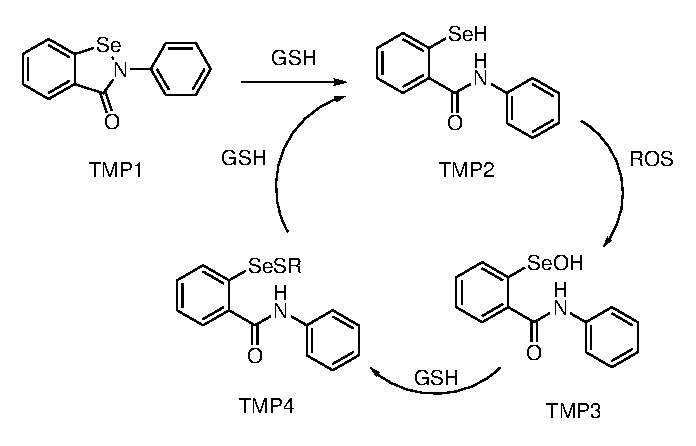
\includegraphics[scale=0.8]{Figures/ebs-cat-cycle.eps}
\caption{Catalytic cycle of ebselen \emph{in vivo}.}
\label{fig:catcycle}
\end{figure}

Molecular modelling is a vital tool in drug development, allowing for rapid and broad-reaching screening of drug candidates against likely substrates at minimal cost and risk.
\emph{Ab initio} quantum methods (QM) are widely used to model small molecules (generally smaller than a few hundred atoms), where their accuracy and ability to describe quantum effects underlying photochemical properties and bond breaking/formation processes are critical.
They are however, computationally costly.
Molecular mechanics (MM), where systems are treated strictly classically, is a viable alternative for large systems.
The drawbacks are that MM relies on having an extensive parameter set (a ``force field'') to describe the system (which is not necessarily available, or applicable to the system at hand), and that descriptions of quantum effects often fail spectacularly.

Both of these issues are encountered when attempting to model ebselen using MM.
Firstly, parameters to describe selenium-containing small molecules are simply not available in most popular force fields, including GAFF, Gromos, and CGenFF.
This has been substantially addressed in the work of Torsello \emph{et al}, where extensive parametrization of a series of diaryl diselenides and diaryl ditellurides was performed, and they provided a methodology to extend this to general chalcogen-containing molecules.\autocite{Torsello2016}
They did not, however, address the second issue of quantum effects, which is reasonable given that they do not play a large role in diselenides.
The chemistry of ebselen, on the other hand, is dominated by the $\sigma$-hole, which is a quantum effect.\autocite{Thomas2015}
The $\sigma$-hole is a region of positive electrostatic potential situated opposite to the Se--N bond, caused by a strongly anisotropic electron distribution around the selenium atom.
This causes the selenium to adopt a highly directional electrophilic character, which can lead to the formation of ``chalcogen-bonds'' with electron pair donors (named by analogy to the ubiquitous hydrogen bond).\autocite{Murray2009}

The presence of a $\sigma$-hole is not a new problem in MM, nor are they exclusive to chalcogens, as they are also found on the heavier halogens, where they give rise to halogen bonding.\autocite{Clark2007}
Perhaps due to the higher prevalence of halogens in drug-like molecules, a number of approaches have been proposed to account for $\sigma$-holes in halogenated molecules.
The common theme in these methods is the inclusion of a pseudoatom with positive electrostatic potential attached to the halogen atom.
This pseudoatom is variously called an extra point (EP), explicit $\sigma$-hole (ESH), or virtual or off-atom centered point, and the approaches differ in the location of the pseudoatom and method used to derive its charge.\autocite{Renidine2011,Ibrahim2011,Hobza2012,Harder2016}
Lone pairs can also be described using negatively charged pseudoatoms, and this approach has been used for some time.\autocite{Dixon1997,Cieplak2001,Harder2016}

It is worth noting an alternative approach, used by Cozzolino and Vargas-Baca, which treats secondary bonding interactions as true bonds, with an explicitly parametrized potential.\autocite{Cozzolino2011}
This was used to parametrize the supramolecular synthon 1,2,5-telluradizaole, which is known to self assemble into a range of interesting structures.
This approach, however, relies on describing the bond using an \emph{an}harmonic potential, which is not easily implemented in AMBER.

The inability to model ebselen in biological systems is a major hurdle in understanding the mechanism of its action. 
In this work we develop a parameter set for the selenium atom in ebselen, including a pseudoatom to simulate the $\sigma$-hole.
This work is implemented in AMBER, due to its popularity, speed, and robustness, although there is no reason these parameters could not be extended to other force fields.
We also restrict ourselves to the ``vanilla'' feature set of AMBER, given that advanced features such as polarizable force fields are not widely used in the analysis of ligand-receptor systems.
We then show that this model accurately reproduces experimental geometries and energies, and compares favourably to \emph{ab initio} calculations.
This force field will prove useful in understanding the interactions between ebselen and current targets, and possibly lead to the discovery of new targets.

\section{Results and Discussion}

We began by deriving the classical bonding parameters involving selenium in ebselen, using the procedure of Torsello.\autocite{Torsello2016}
All quantum calculations were performed using Gaussian09, unless otherwise specified.\autocite{Gaussian09}
Electrostatic potentials were calculated using the \texttt{cubegen} program in the Gaussian suite, or \texttt{mol2cub}\footnote{\url{https://github.com/tjfellowes/mol2cub}}.
The ground state geometry of ebselen was optimized at the $\omega$B97X-D/def2TZVP level, followed by vibrational analysis to confirm the structure was minimized.\autocite{Chai2008,Weigend2005,Weigend2006}
Partial charges were assigned to the atoms using the RESP scheme, at the HF/6-31G* level.\autocite{Cornell1993}
This was chosen for consistency with existing AMBER force fields.

\subsection{Classical bonding parameters}
Bond and angle force constants were derived by conducting a relaxed potential energy surface scan over a range of $\pm0.3$~\AA~for bonds and $\pm10$\degree~for angles.
The resulting data was truncated to within 5~kcal/mol of the equilibrium energy (at larger distances the surfaces were appreciably anharmonic), and this surface was fitted with a classical harmonic oscillator model (equation \cref{eqn:cho}) using the \texttt{nls} function in the R software package.\autocite{R}
The equilibrium distance/angle $x_0$ was fixed to the value from the optimized geometry.
Torsion angles were similarly scanned at the DFT and MM (with the torsion term set to zero) levels, and the difference between these surfaces was fitted using a periodic series truncated to the fourth order (equation \cref{eqn:dihe}).
An unrealistically high torsion barrier was identified in the central \ce{Se-N-C_{ar}-C_{ar}} dihedral, due to a repulsive short-range interaction between the aromatic hydrogen and carbonyl oxygen.
We were unable to correct for this in the periodic series describing the torsion, so the non-bonding parameter for the oxygen was reduced to ???.
This did not appear to have any negative impact on interactions involving this oxygen, while improving the overall structural model.
The resulting parameters are presented in \cref{tab:cho-params,tab:dihe-params}.

\begin{equation}
    V(x) = \frac{1}{2} k (x - x_0) ^2
    \label{eqn:cho}
\end{equation}

\begin{equation}
    V(\phi) = \sum_{n=1}^4 \left( \frac{V_{\mathrm{max},n}}{2} \times (1 + \cos(n \phi + \gamma_n)) \right)
    \label{eqn:dihe}
\end{equation}

\begin{table}
    \centering
\begin{tabular}{lll}\toprule
         Parameter & $x_0$ & $k$  \\\midrule
         r(\ce{Se-N}) & 1.8586 & 434.67 \\
         r(\ce{Se-C}) & 1.8829 & 422.33 \\
         $\angle$(\ce{C-Se-N}) & 86.6 & 610.7 \\
         $\angle$(\ce{Se-N-C_{ar}}) & 119.6 & 182.7 \\
         $\angle$(\ce{Se-N-C_{CO}}) & 115.8 & 404.5 \\
         $\angle$(\ce{C-C-Se}) & 119.4 & 329.2 \\
         \bottomrule
    \end{tabular}
    \caption{Classical parameters for ebselen. Bond lengths are given in \AA, and angles in degrees. Force constants are given in kcal/mol$\cdot$\AA$^2$ or kcal/mol$\cdot$radian$^2$.}
    \label{tab:cho-params}
\end{table}

\begin{table}
    \centering
    \footnotesize
    \begin{tabular}{lllllllll}\toprule
         Parameter & $V_\mathrm{max,2}$ & $V_\mathrm{max,4}$& $V_\mathrm{max,6}$& $V_\mathrm{max,8}$& $\gamma_2$ & $\gamma_4$ & $\gamma_6$ & $\gamma_8$ \\
         & kcal/mol & kcal/mol & kcal/mol & kcal/mol & \degree & \degree & \degree & \degree\\\midrule
         $\phi$(\ce{C_{ar}-C_{ar}-N-Se}) & -0.0862 & 0.7841 & 0.0363 & 0.0424 & 180 & 0 & 0 & 0 \\
        \bottomrule
    \end{tabular}
    \caption{Dihedral parameters for ebselen. NEEDS REVISION}
    \label{tab:dihe-params}
\end{table}

Values of 2.12 and 0.2910 for the Lennard-Jones parameters $\sigma$ and $\varepsilon$ were used for selenium.
The default GAFF Lennard-Jones parameters for the carbonyl oxygen were found to give an unreasonably high barrier to rotation about the central dihedral angle (due to steric repulsion between the oxygen and the aryl hydrogen), so they were changed to 1.25 and 0.2.

Default GAFF values were used for all other atoms, and Lorentz/Berthelot mixing rules were used to derive cross-terms.

\subsection{Energy decomposition analysis}
While attempting to model the $\sigma$-hole using molecular mechanics, we must remember that we are forcing a classical treatment onto an inherently quantum phenomenon.
That said, some parts of the quantum phenomenon are easier than others to treat classically.
There are thought to be three attractive energetic components which contribute to a $\sigma$-hole interaction.
Namely, electrostatics, induction, and dispersion.\autocite{Bleiholder2006,Bleiholder2007,Pascoe2017}
The magnitudes of each component of $\sigma$-hole interactions has been the subject of heated debate in recent years.
For many applications, these disagreements are fairly philosophical and of little consequence, however this is not the case when attempting to model $\sigma$-hole interactions using MM.

The electrostatic component generally refers to the interaction between two static (not distorted by each other) electric fields, which can be graphically represented by visualizing the electrostatic potential surfaces of the donor and acceptor moieties (\cref{fig:ebs-esp}).
This is already treated in MM (for the case of atom centered charges) as a sum of pairwise interactions. 
The accuracy of this component is only limited by the resolution of the electrostatic potential; it would appear that a pseudoatom approach could thus adequately describe the $\sigma$-hole.
Dispersion is accounted for empirically within the $r^{-6}$ term of the Lennard-Jones potential.

Issues arise when attempting to model the induction component of the $\sigma$-hole $E_{\mathrm{ind}}$.
This component refers to the redistribution of charge within (polarization) or between (charge-transfer) the donor and acceptor as they approach each other.
Movement of charge is simply not accounted for within the most common AMBER force fields.
This presents a large problem, as charge-transfer drives the strong directionality of $\sigma$-hole interactions, and may account for a significant proportion of their strength.

To ensure that this is not an insurmountable problem for this parametrization, we conducted energy decomposition analyses (EDA) on a variety of complexes containing ebselen.
There are numerous EDA schemes available such as KM-EDA, NEDA, and ALMO, however we chose to use symmetry-adapted perturbation theory (SAPT).\autocite{SAPT2020,Jeziorski1994PerturbationComplexes}
In contrast to several other schemes, SAPT explicitly includes dispersion (as opposed to adding it as an empirical correction), and contains no physically meaningless ``catch-all'' energy term.
The total interaction energy $E_\mathrm{tot}$ is decomposed into an electrostatic component $E_\mathrm{elst}$, an inductive component $E_\mathrm{ind}$ (this incorporates polarization and charge transfer, as they are not distinct phenomena within the SAPT framework), and a dispersive component $E_\mathrm{dis}$.
These attractive forces are balanced by a repulsive exchange component $E_\mathrm{exch}$.

Four Lewis bases were chosen which are representative of those likely to be encountered in biological systems, and which span a wide range of basicity.
Their structures are given in \cref{fig:complexes}.
SAPT(DFT) analyses were conducted using the Psi4 software package on geometries optimized at the $\omega$B97X-D/def2TZVP level, and the results are shown in \cref{fig:eda}.\autocite{Parrish2017}

\begin{figure}
    \centering
    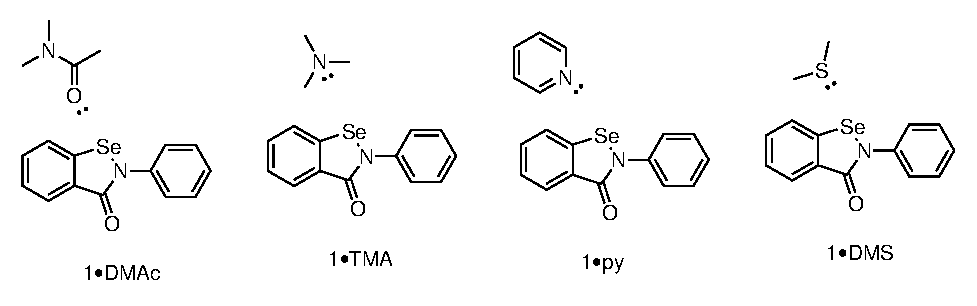
\includegraphics[scale=0.8]{Figures/sapt-complexes.eps}
    \caption{Structures of complexes used for SAPT(DFT) analysis.}
    \label{fig:complexes}
\end{figure}

\begin{figure}
    \centering
    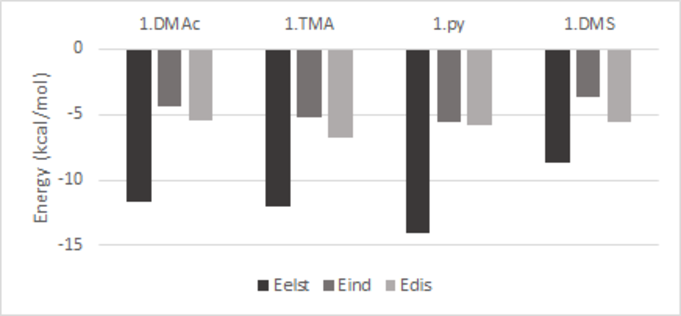
\includegraphics[width=0.5\linewidth]{Figures/sapt-eda.pdf}
    \caption{SAPT(DFT) analysis of complexes with four Lewis bases. All energies are given in kcal/mol.}
    \label{fig:eda}
\end{figure}

The SAPT results indicate that the majority (around 80\%) of the interaction can be described by electrostatics and dispersion.
This suggests that the explicit $\sigma$-hole parametrization will be reliable, as electrostatics and dispersion are well described by MM.

\subsection{Incorporation of pseudoatom}
With classical parameters for ebselen in hand, as well as theoretical assurance that the system can be adequately described using electrostatics, we began to optimize parameters for the pseudoatom representing the $\sigma$-hole.
While AMBER supports massless extra points (which would be ideal to model the $\sigma$-hole), these are necessarily hardcoded into the program at this stage. We determined that modification of core routines and recompiling the code was beyond the scope of this work, and represented a significant hurdle to other groups wishing to adopt our model.
The pseudoatom was therefore modelled as a H atom, with an associated mass of 1 amu.
The SHAKE algorithm is applied to all H atom types, which serves to damp high frequency vibrations and allows longer time steps to be used.
The VDW parameters for this atom type were set to 0, so it would only exert influence through the electrostatic force.
It is important to note that the non-zero mass of the pseudoatom will slightly effect the dynamics of the system, but not the final equilibrium.
The pseudoatom was placed on the selenium atom 180\degree~from the nitrogen, at a distance of 0.8~\AA~(i.e. within the VDW surface).
Force constants of 119.2~kcal/mol$\cdot$\AA$^2$ and 150.0~kcal/mol$\cdot$radian$^2$ were applied. 
The former was chosen to mimic the polarizability of an isolated selenium atom, and the latter was arbitrarily set.
By employing a finite force constant, we are able to simulate the polarization contribution to Ch-bonding.
The polarizability of an atom can be approximately calculated from first principles as
\begin{equation}
\alpha_{\mathrm{atom}} = 4 \pi \epsilon_0 r^{3}
\end{equation}
where $r$ is the atomic radius.
The polarizability of a dipole with variable length (such as the polarized Se--pseudoatom bond) can be shown to be
\begin{equation}
    \alpha_{\mathrm{dipole}} = \frac{q^2}{k}
\end{equation}
where $q$ is the charge separation and $k$ is the force constant.
Equating these expressions and solving for $k$ gives a force constant of 119.2~kcal/mol$\cdot$\AA$^2$.

\subsection{Electrostatic potential map}
With these parameters in hand, we were able to construct electrostatic potential maps (\cref{fig:ebs-esp}), which show good qualitative agreement between the DFT and pseudoatom model potentials.
Barely visible in the DFT ESP map is a second $\sigma$-hole, opposite the Se--C bond.
Carbon is significantly less electronegative than nitrogen, so it doesn't polarize the selenium to the same degree, leading to a much smaller $\sigma$-hole.
While it is conceivable that this $\sigma$-hole could form Ch-bonds as well, we have not observed any evidence of this in any of the derivatives we have studied.\autocite{Fellowes2019} 
We therefore did not attempt to model it, although it could be modelled in the same way as the main $\sigma$-hole opposite the nitrogen.

\begin{figure}
    \centering
    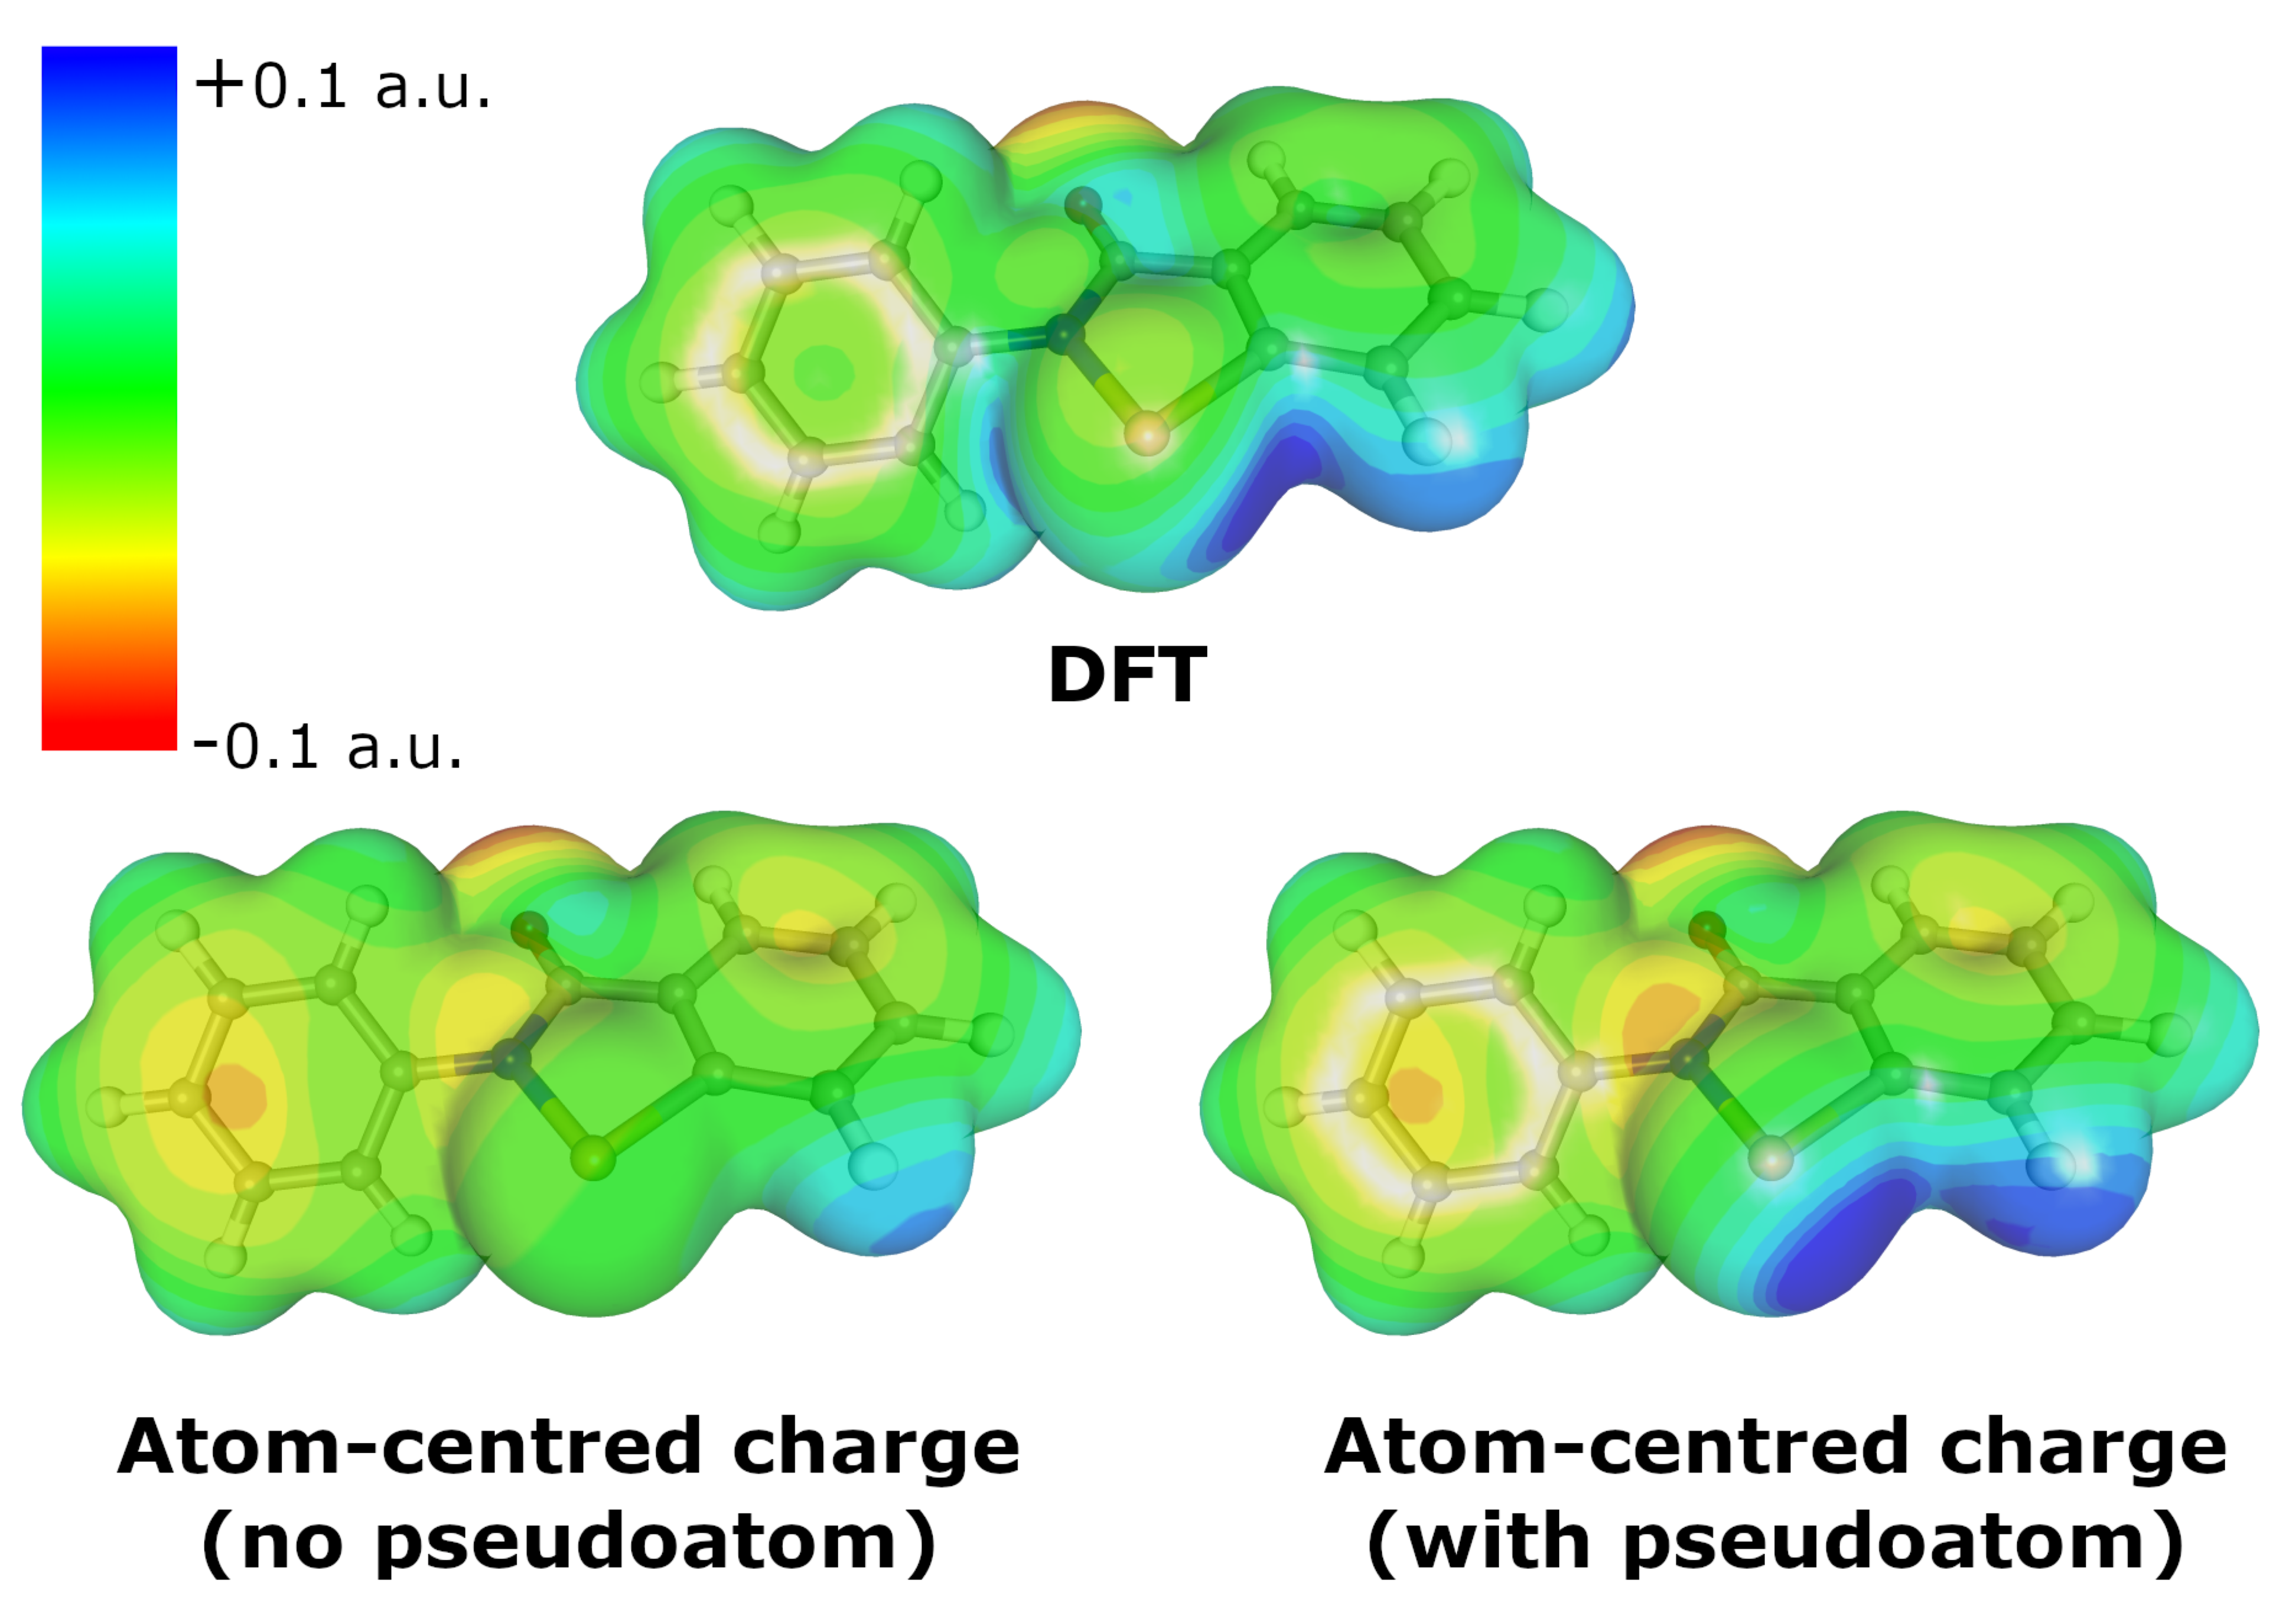
\includegraphics[width=0.5\linewidth]{Figures/mm-dft-esp.pdf}
    \caption{ESP mapped on the 0.005~a.u. electron density isosurface. The $\sigma$-hole is visible as the dark blue region on the DFT and atom-centered charge (with pseudoatom) surfaces.}
    \label{fig:ebs-esp}
\end{figure}

\subsection{Validation against DFT geometries}
A preliminary verification of our model was conducted by comparing the geometries and energies calculated in the SAPT(DFT) analysis with the respective MM values.
The Lewis bases chosen for the SAPT(DFT) analysis were constructed in AMBER.
GAFF was used for all atoms, and an extra point was added to simulate the lone pair per the method of Dixon and Kollman.\autocite{Dixon1997}
Geometries were assessed by minimizing the ebselen-Lewis base structure over 1000 steps, then conducting a 2~ns MD trajectory in a vacuum.
Trajectories were performed at 300~K for the strongly bonded systems (\cmpd{ebs}$\cdot$py and \cmpd{ebs}$\cdot$DMAc), however the weaker complexes (\cmpd{ebs}$\cdot$TMA and \cmpd{ebs}$\cdot$DMS) tended to dissociate under these conditions.
Their trajectories were therefore conducted at 200~K and 100~K respectively.
Binding energies were calculated by slowly cooling the system to 0~K, then conducting a short simulation to determine the potential energy of the system.
Relevant parameters are given in \cref{fig:1.py-geom} and \cref{tab:ebs-geom}, alongside DFT values for comparison.

\begin{figure}
    \centering
    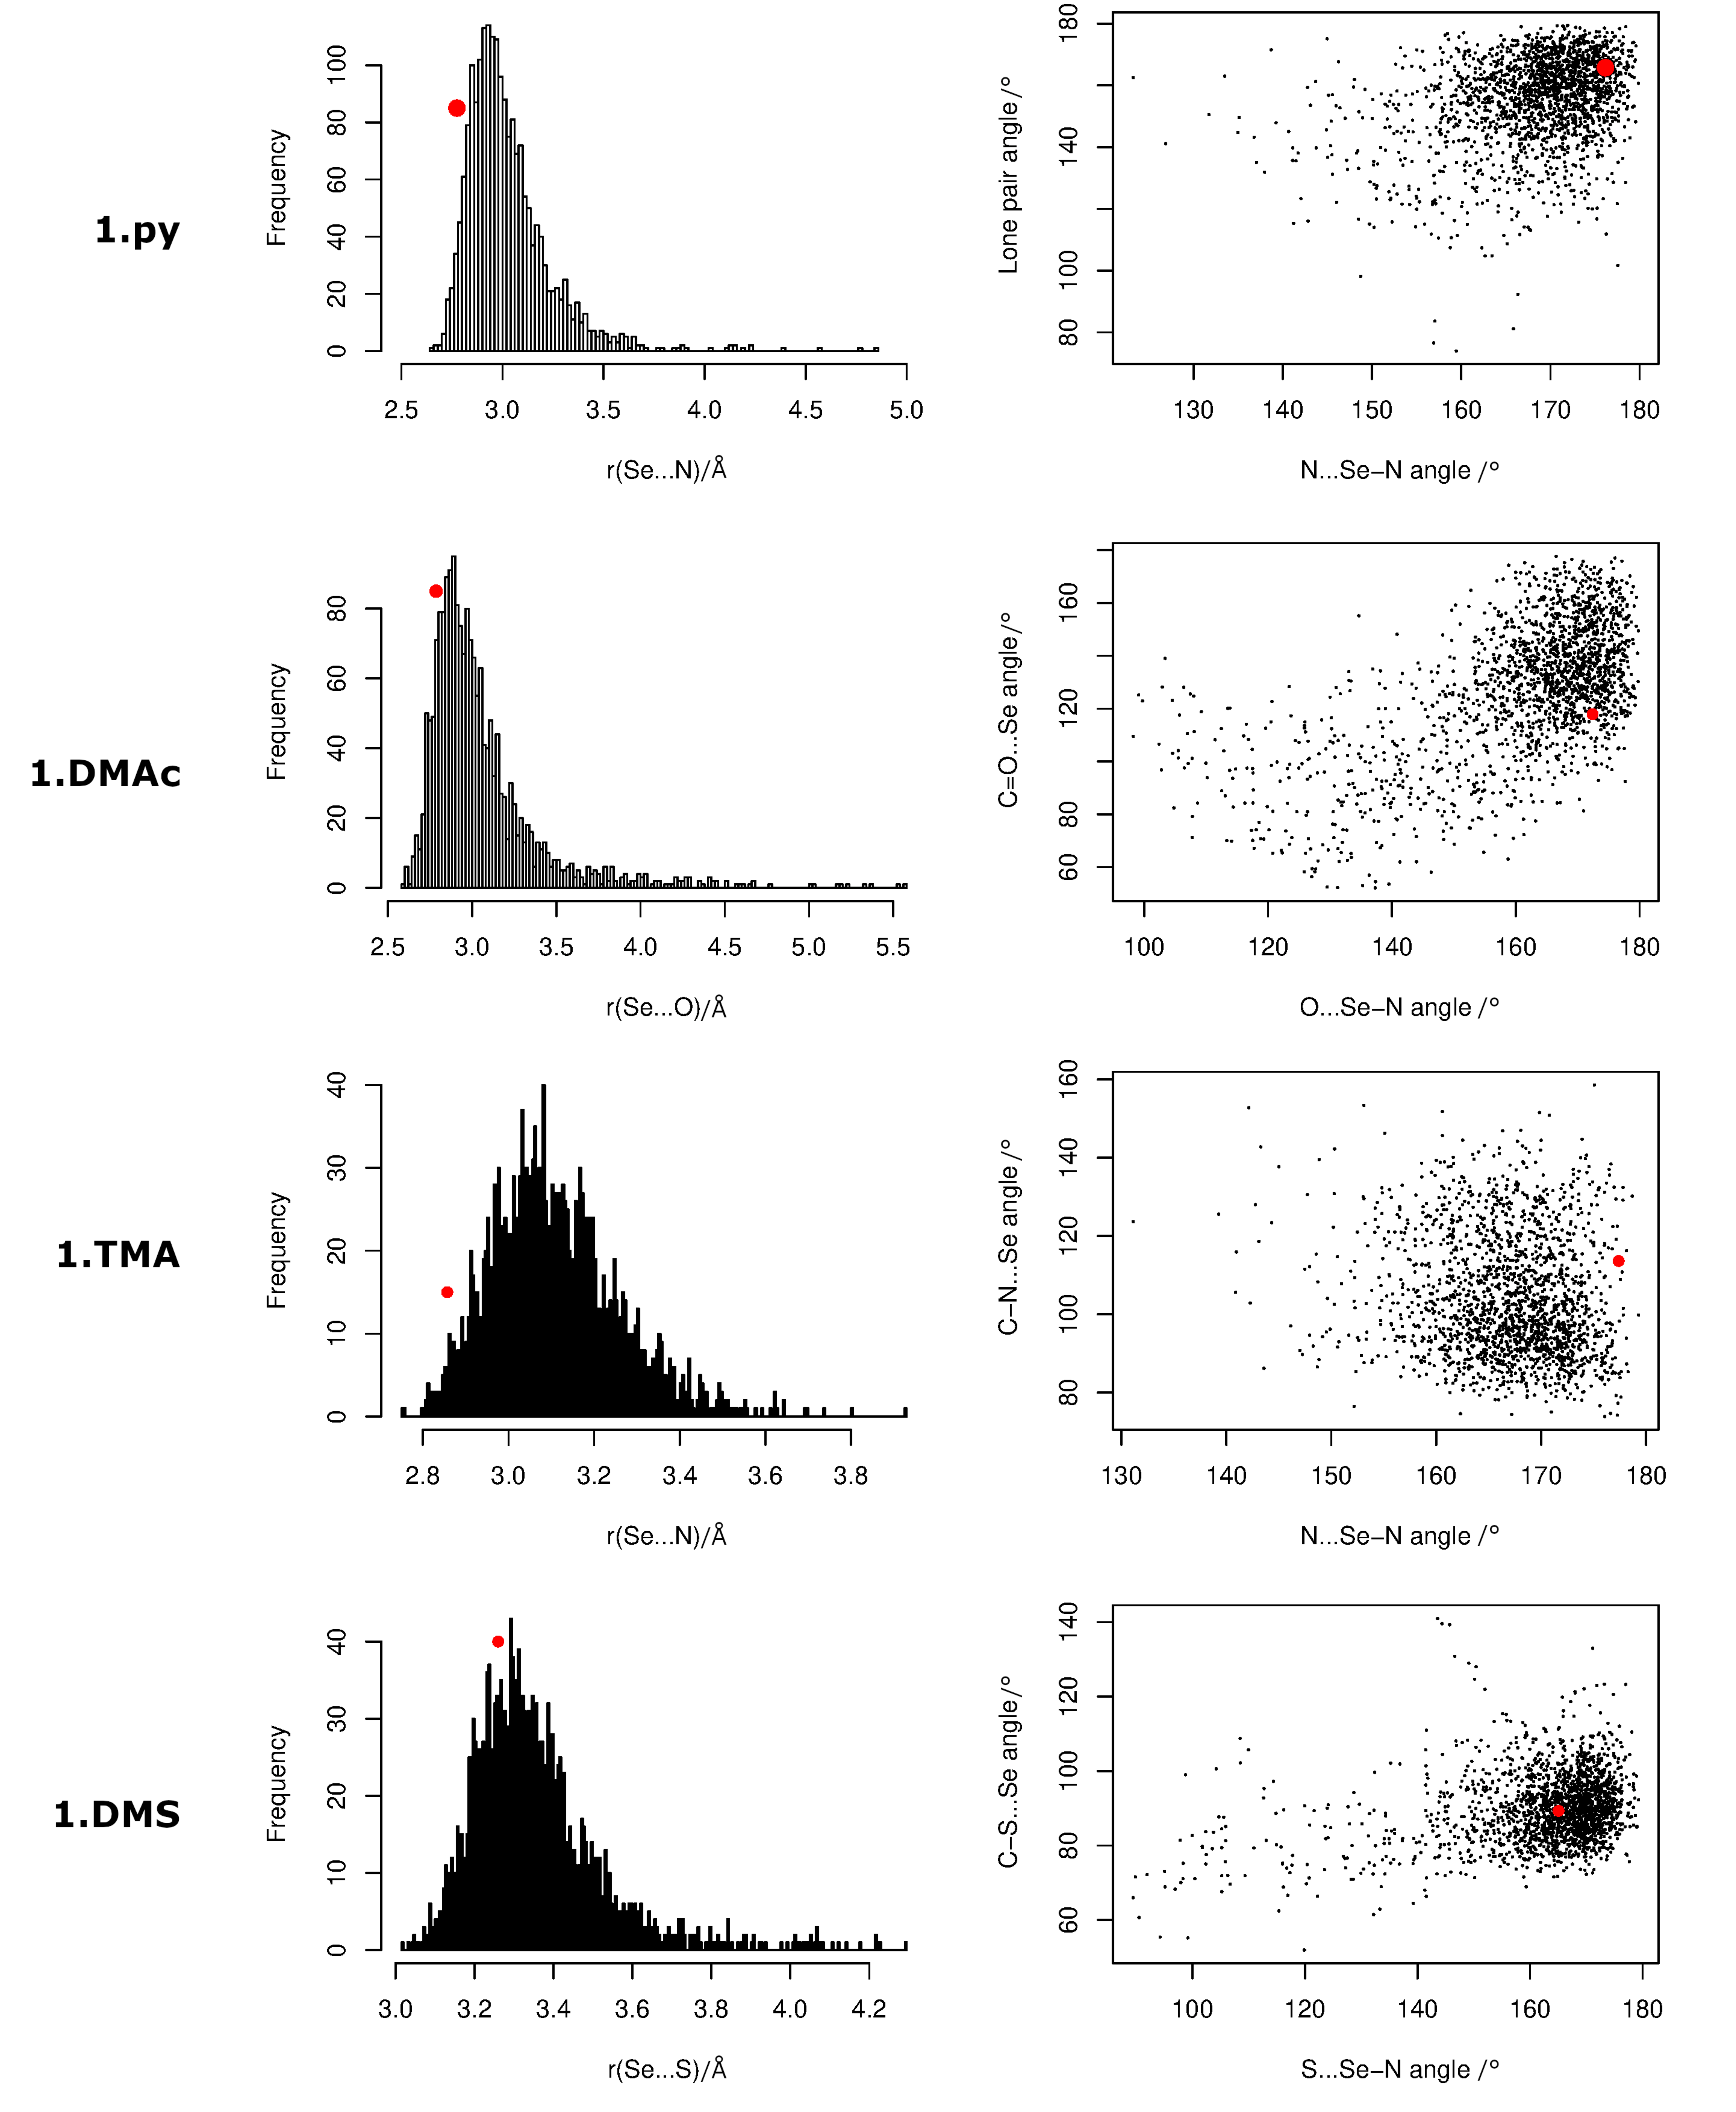
\includegraphics[width=\linewidth]{Figures/geom-distribution.pdf}
    \caption{Distribution of geometric parameters for complexes over a 2~ns trajectory. DFT equilibrium values are shown as red circles. REDO}
    \label{fig:1.py-geom}
\end{figure}

\begin{table}
    \centering
    \begin{tabular}{lllll}\toprule
        Complex & r(\ce{Se\cdots B}) & $\angle$(\ce{N-Se\cdots B}) & $\angle$(lone pair) & Energy \\ & & & & (kcal/mol)\\\midrule
        \cmpd{ebs}$\cdot$py & 2.98~\AA~(2.775~\AA) & 169.8\degree~(176.2\degree) & 158.2\degree~(165.7\degree) & -8.376 (-7.093) \\
        \cmpd{ebs}$\cdot$DMAc & 2.964~\AA~(2.786~\AA) & 166.3\degree~(172.4\degree) & 129.7\degree~(117.9\degree) & -10.351 (-7.551) \\
        \cmpd{ebs}$\cdot$TMA & 3.091~\AA~(2.857~\AA) & 167.6\degree~(177.4\degree) & 100.71\degree~(113.6\degree) & -6.666 (-6.627) \\
        \cmpd{ebs}$\cdot$DMS & 3.322~\AA~(3.265~\AA) & 165.0\degree~(177.4\degree) & 89.1\degree~(89.8\degree) & -4.541 (-5.646) \\
        \bottomrule
    \end{tabular}
    \caption{Median geometric parameters for complexes with \cmpd{ebs}. DFT equilibrium values are given in brackets for comparison. DFT energies are derived from SAPT(DFT). REDO}
    \label{tab:ebs-geom}
\end{table}

\subsection{Validation against experimental melting point}
We also sought to validate our model against the experimentally determined melting point.
An ebselen crystal (CSD code \textbf{SENGOH}, $5 \times 5 \times 5$ unit cells, 1000 molecules) was constructed, and placed in a simulation box of the appropriate size at 1~atm.
The crystal was heated to 300K, then 5 random molecules were deleted to create voids (crystal defects) that act as nucleation sites for melting.
This avoids the effects of superheating, which is a documented issue in simulated phase transitions.\autocite{???}
The nucleated geometry was used as a starting point for a series of trajectories at temperatures from 400--500~K in 10~K increments to identify an approximate melting range, then 1~K increments to accurately determine the melting point.

\begin{figure}
    \centering
    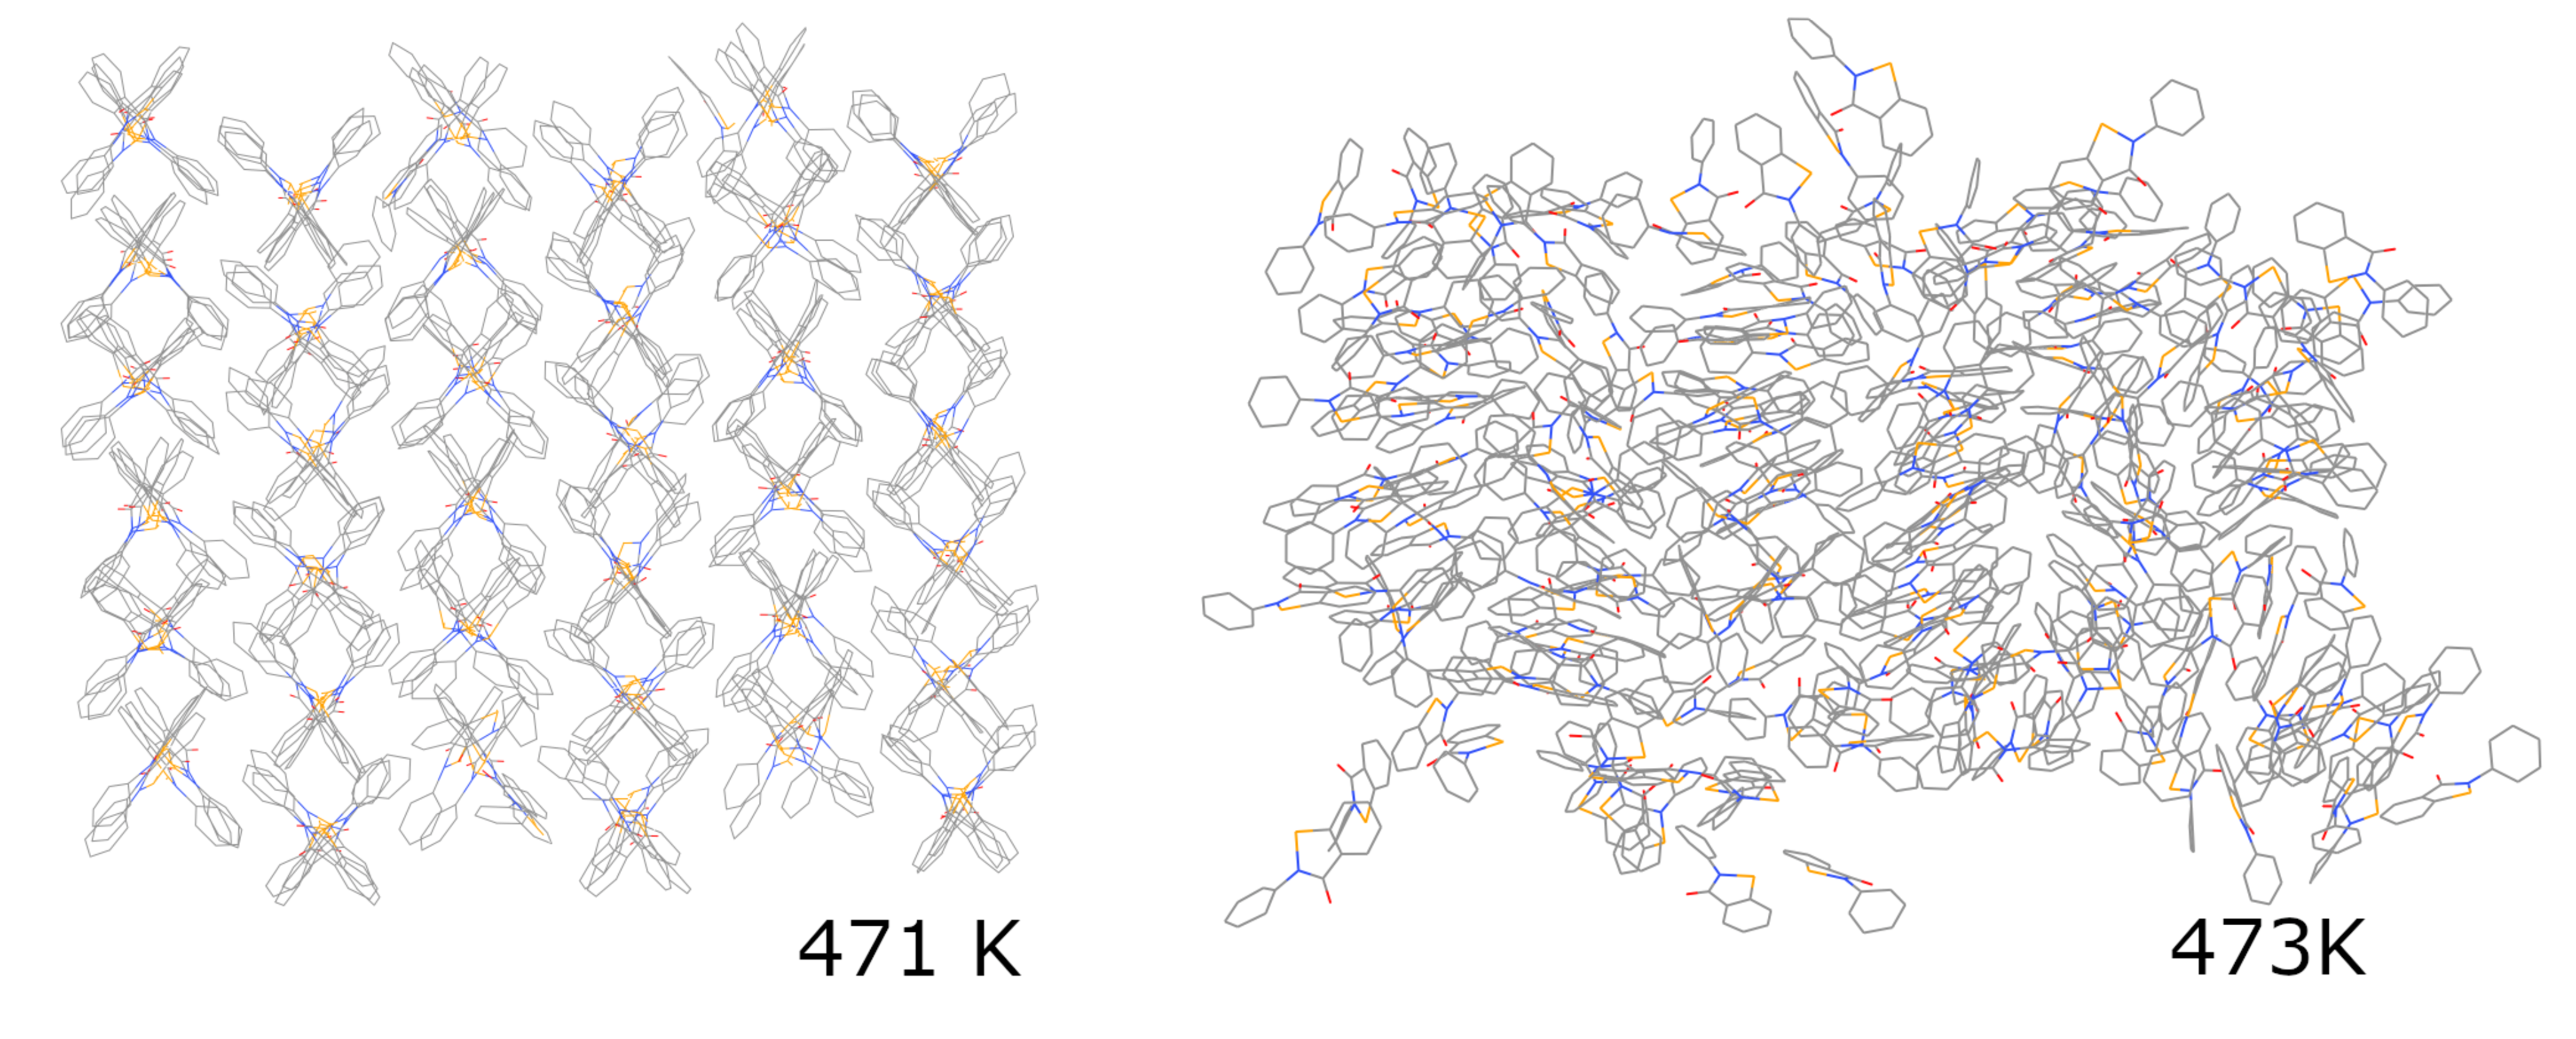
\includegraphics[width=\columnwidth]{Figures/melting.pdf}
    \caption{Melting of a simulated ebselen crystal. The final state of the crystal is shown after 2~ns at the specified temperature.}
    \label{fig:melting}
\end{figure}

These results show that Ch-bonds can be adequately described by the inclusion of a positively charged pseudoatom.
Interestingly, the weaker complexes (\cmpd{ebs}$\cdot$TMA and \cmpd{ebs}$\cdot$DMS) are better described both in terms of geometry and energy.
This may be due to the somewhat decreased charge-transfer component of these interactions, which is poorly described.
For the stronger complexes, both the interaction energy and distance are overestimated, representing a compromise between the two criteria.

\subsection{Validation against SOD1 binding}
In order to show the utility of our model, we conducted a binding simulation with a known ebselen target.
Superoxide dismutase-1 (SOD1) forms a covalent complex with ebselen through the Cys111 residue, which appears to support correct folding of the protein, inhibiting aggregation and associated toxicity.\autocite{Capper2018}
Although formation of the covalent complex cannot be simulated using our model (as this is a bond-forming process), we are able to visualize the stabilized encounter complex which undergoes ring opening to form the final adduct.
Indeed, the Ch-bond formed through the $\sigma$-hole can be thought of as the early stages of a nucleophilic attack at the selenium.\autocite{Thomas2015}
SOD1 (PDB \textbf{2C9V}) was chosen because of the availability of an atomic resolution structure, demonstrated evidence of ebselen binding, and it's relatively small size.\autocite{Capper2018,Strange2006}
The structure was prepared for AMBER by removing disorder, then removing water and ions (the Cu and Zn ions were retained).
The ff14SB force field was used for the protein.
The ebselen residue was introduced within the binding groove approximately halfway between the two units.
The complex was then neutralized by addition of four \ce{Na+} ions at the sites of most negative electrostatic potential, and solvated with a TIP3P explicit water model to give a final box size of $77.095\times 96.253\times 78.411$\AA.
The structure was minimized over 1000 cycles to remove bad contacts, then heated to 300~K over 200~ps.
A simulation of 2~ns at 300~K was then performed to assess the average binding geometry, which was found to exhibit a bifurcated Ch-bond between the expected Cys111 sulfur and the adjacent Ile113 backbone carbonyl (\cref{fig:sod1-ebs}).
A similar experiment was performed \emph{without} the $\sigma$-hole, which failed to bind in a reproducible geometry, with the ebselen molecule wandering through the groove.
This is presumably driven by hydrophobic interactions, and the entropic cost of desolvation.

\begin{figure}
    \centering
    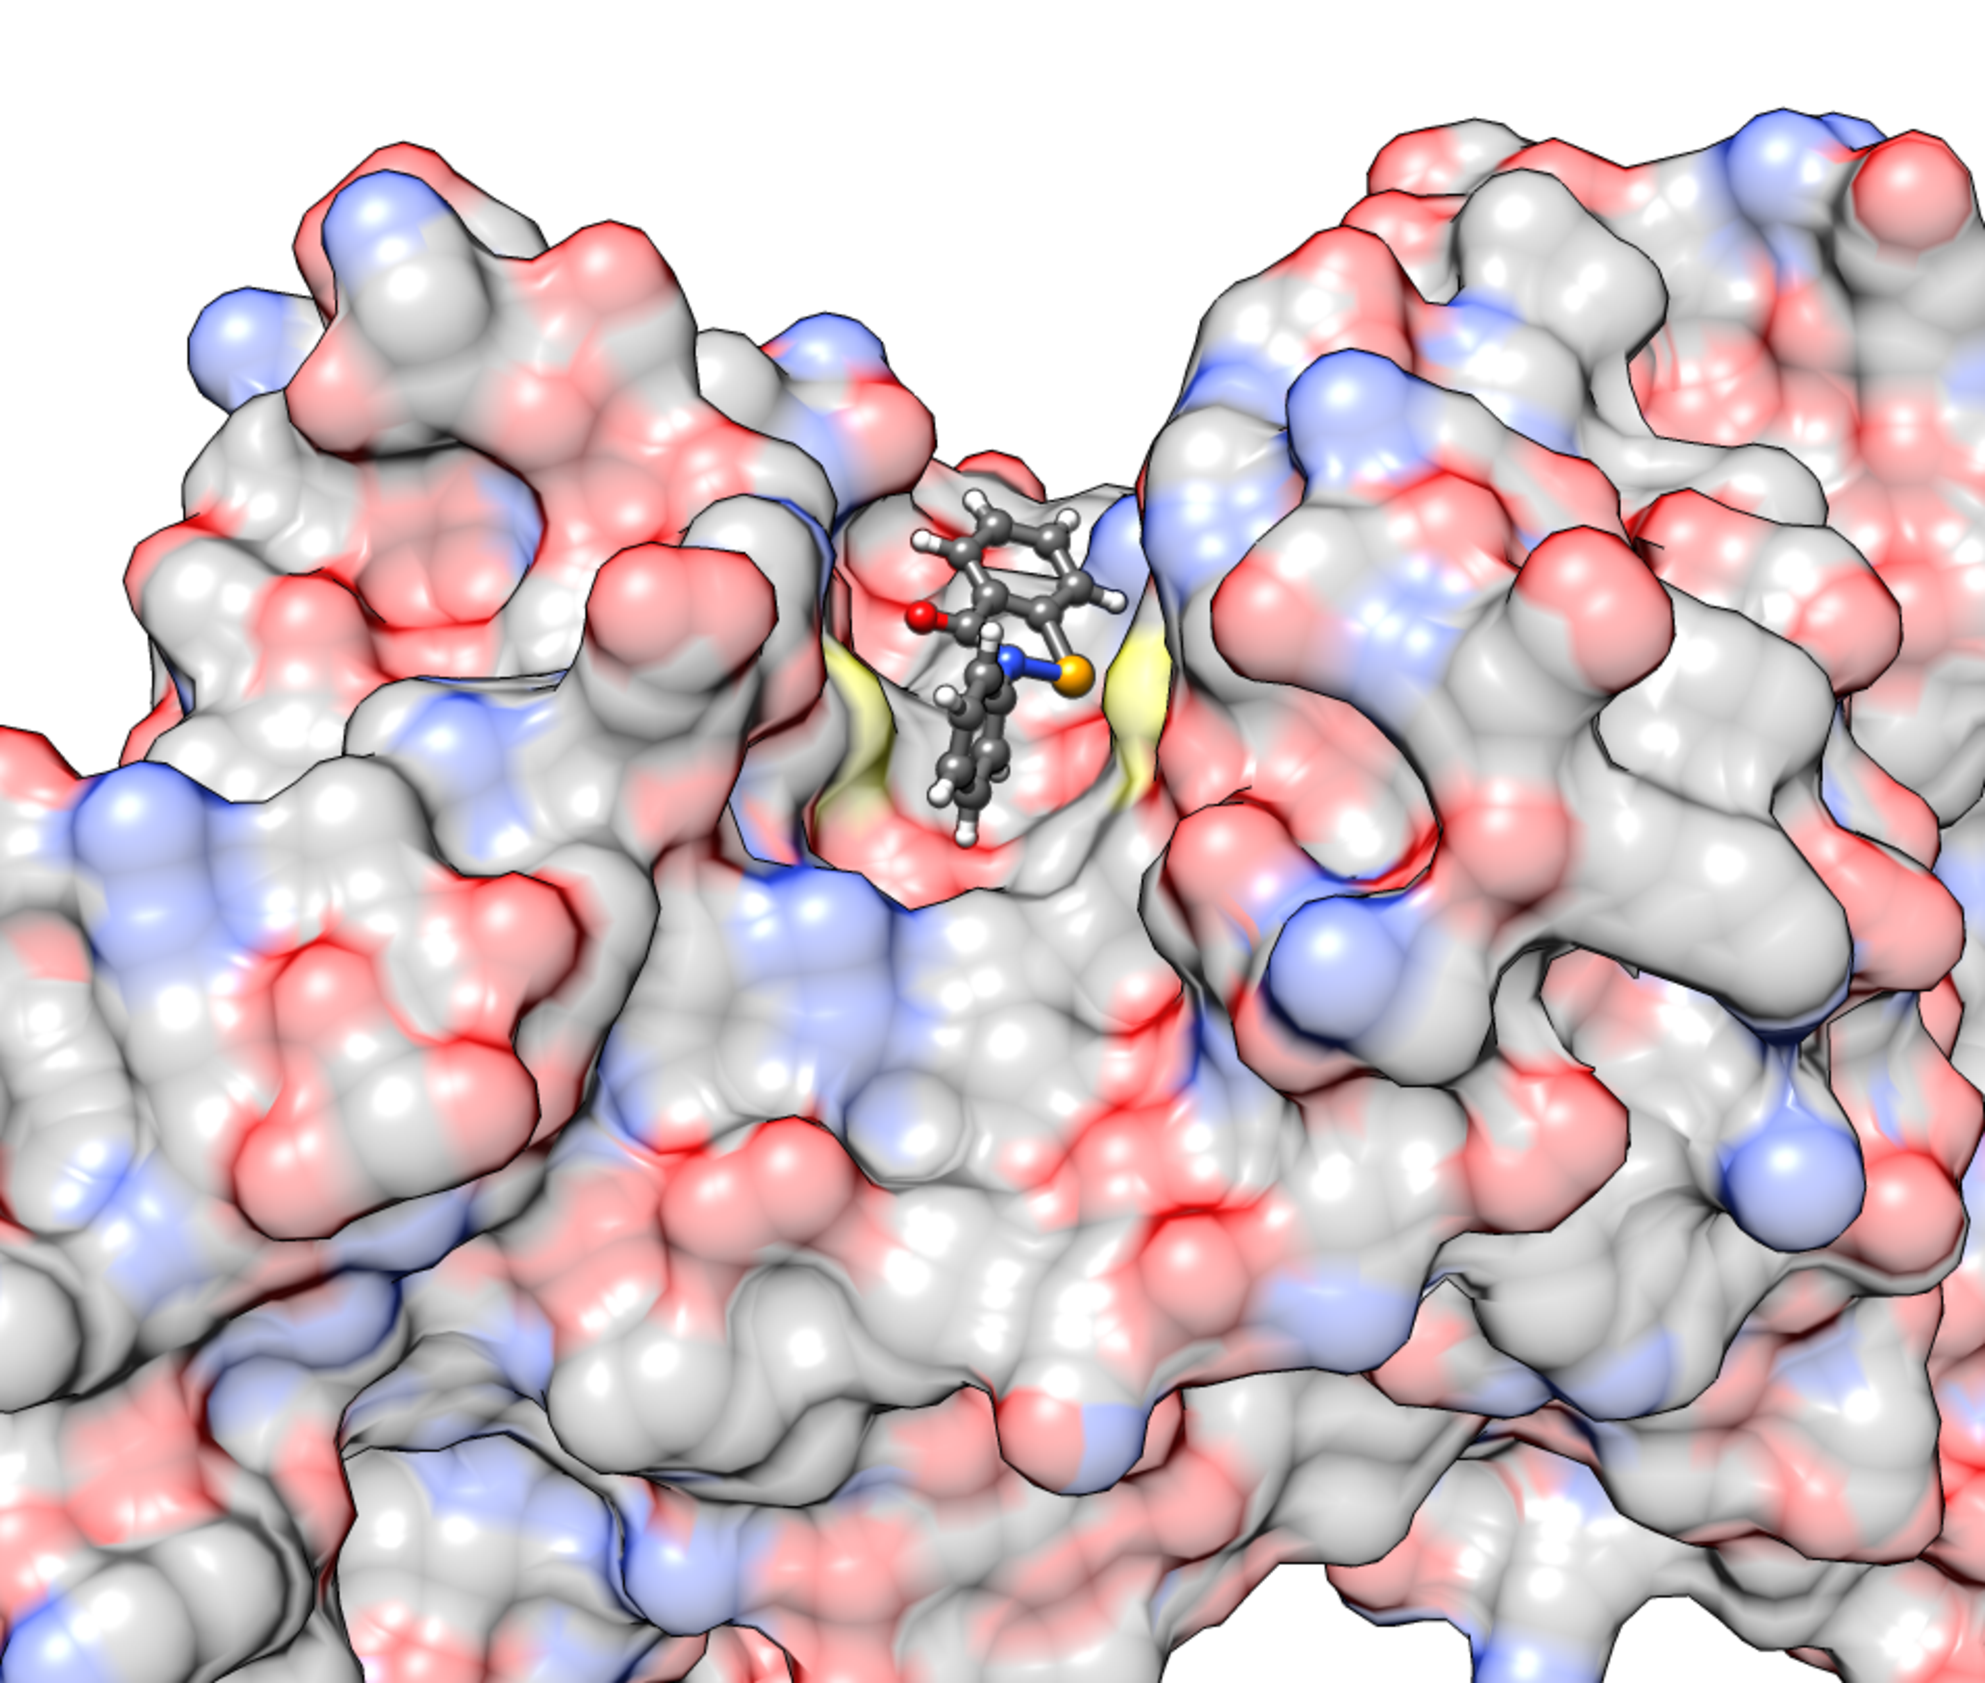
\includegraphics[width=0.45\linewidth]{Figures/sod1-ebs-a.pdf}
    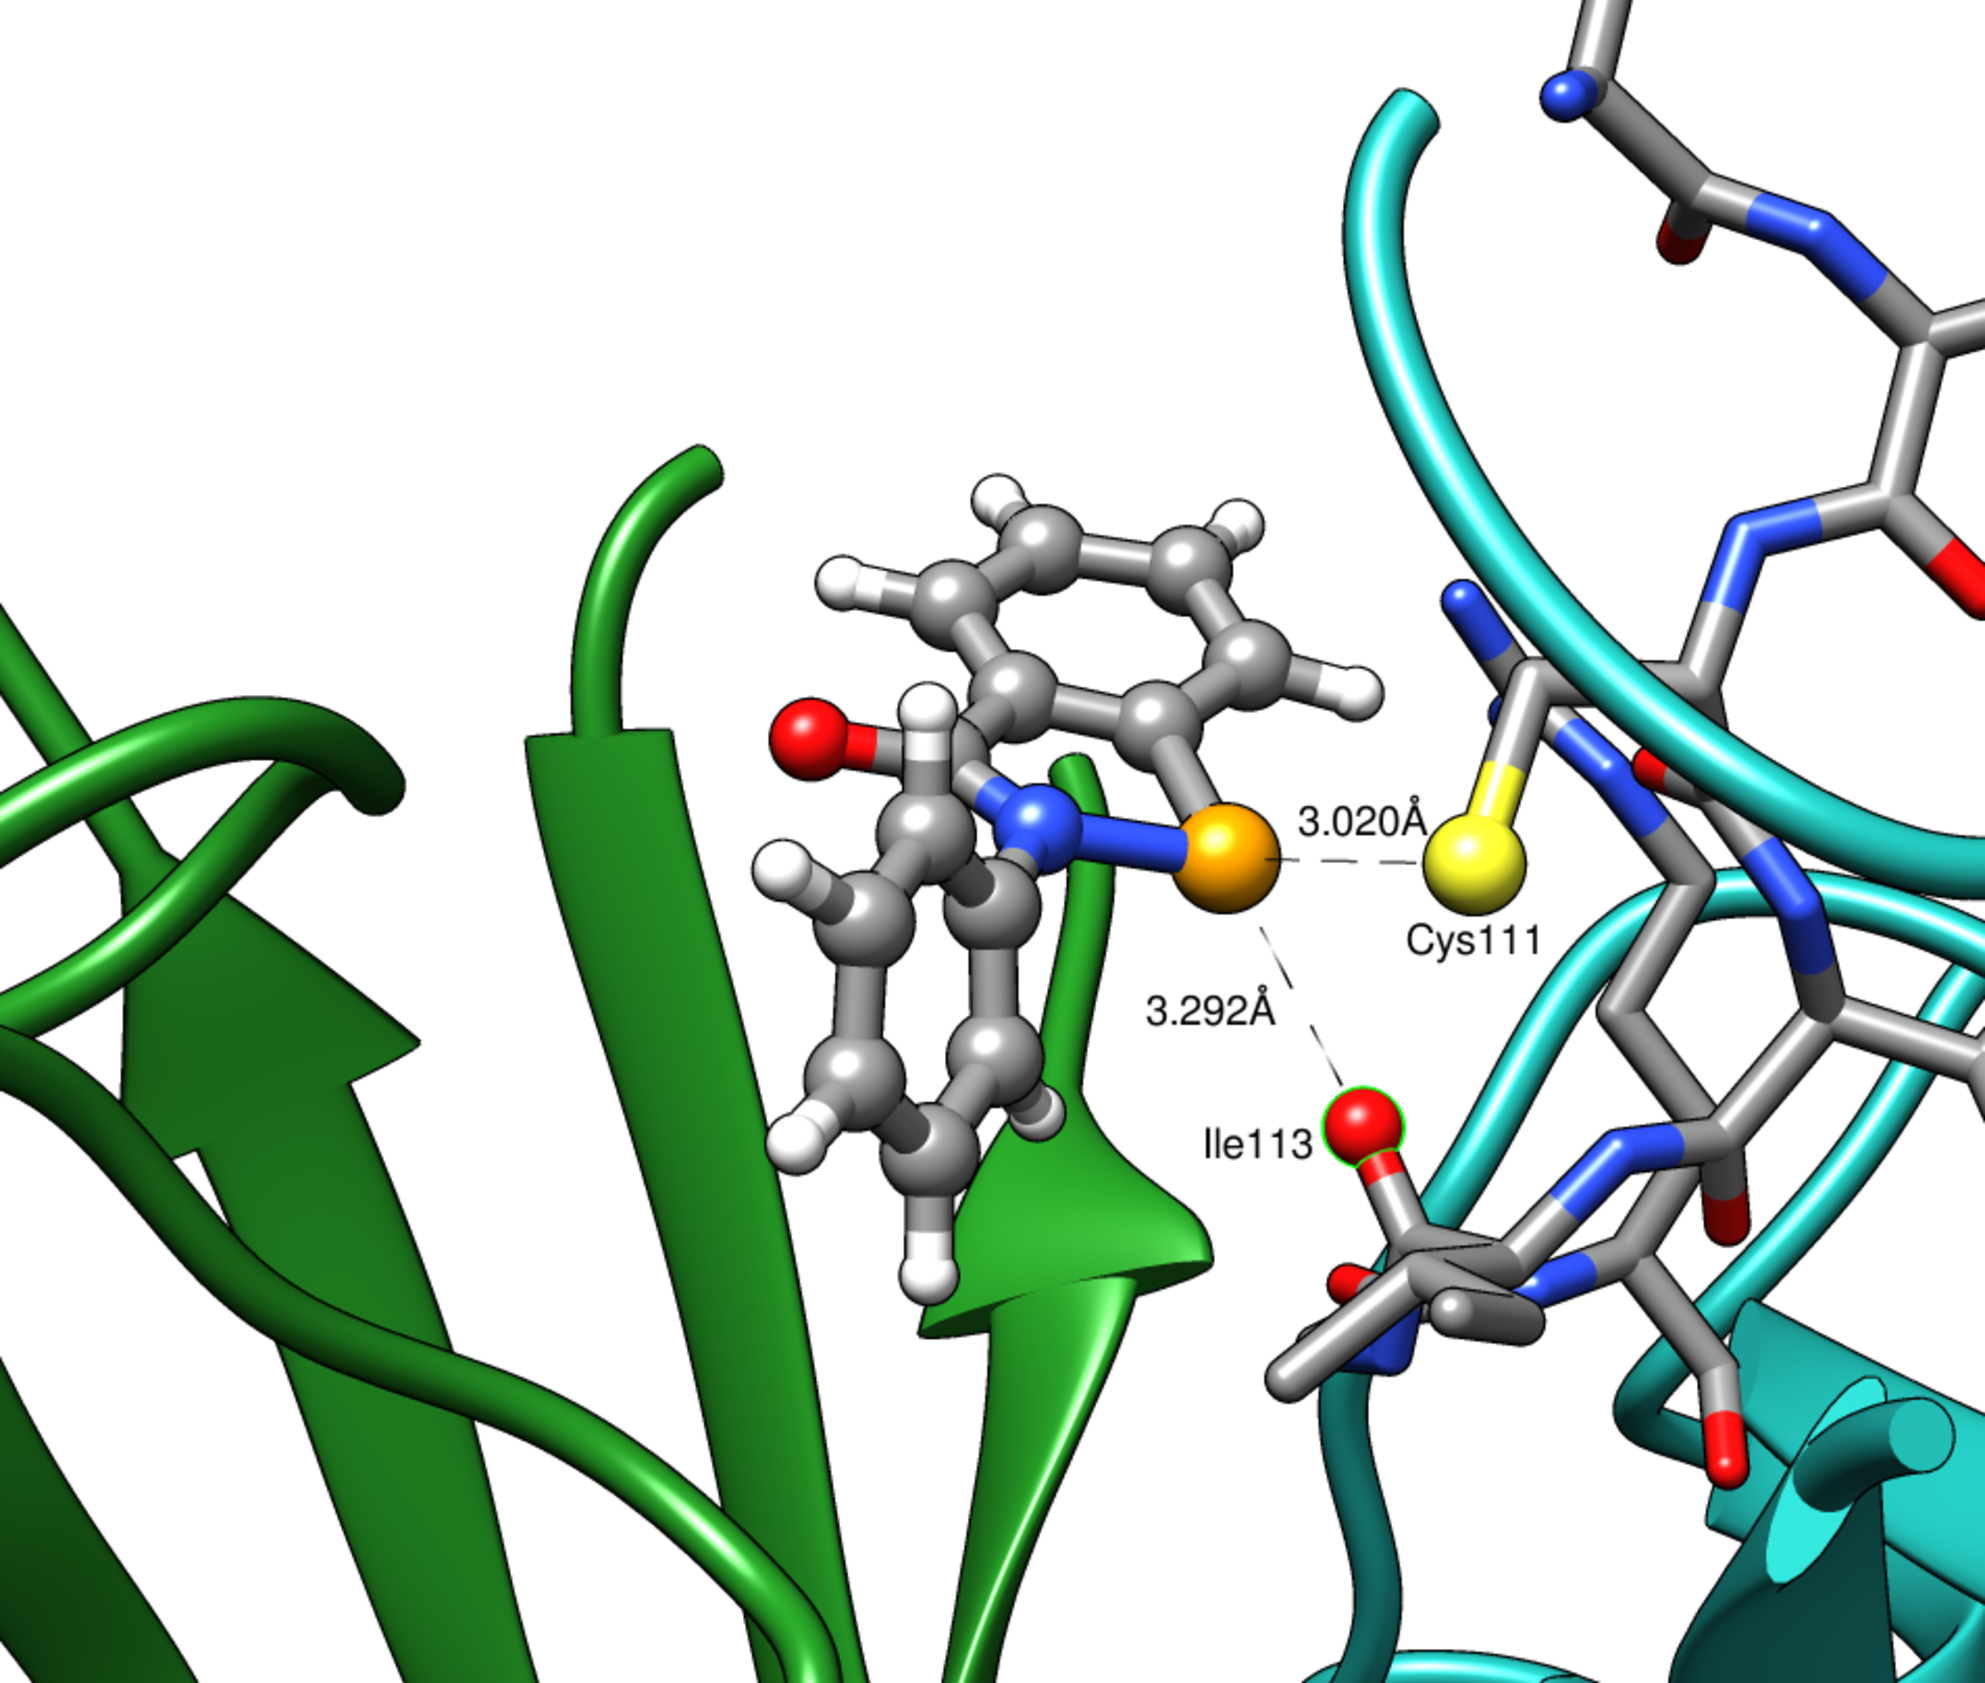
\includegraphics[width=0.45\linewidth]{Figures/sod1-ebs-b.pdf}
    \caption{Average binding geometry of ebselen in the SOD1 groove.}
    \label{fig:sod1-ebs}
\end{figure}

\section{Conclusion}
In conclusion, we have developed a set of parameters which can greatly improve modelling of ebselen and its derivatives.
Our model gives realistic geometries and energies of gas phase complexes, and reproduces the interaction between ebselen and a protein.
Although this work is restricted to ebselen itself, the parameters will be generally applicable to derivatives of ebselen (with appropriate charge fitting).
We hope that these results will be useful for the discovery of new targets.

\printbibliography[heading=subbibliography]
\end{refsection}